% !TeX root = ../document.tex
\documentclass[../document.tex]{subfiles}
\lstset{inputpath=sections}
\begin{document}

	\subsection{Logistic regression}

	\paragraph{logistic model}
	A linear model can't guarantee that the predicted response will be between 0 and 1. Hence the idea is to use the logistics function, which goes in an S-shape smoothly from 0 to 1 and model its argument using a linear model.
	\begin{equation}
		p(X)=\frac{e^{\beta_{0}+\beta_{1}X}}{1+e^{\beta_{0}+\beta_{1}X}}
	\end{equation}
	One problem that is left to solve is, how the coefficient can be found so that this will generate a meaningful curve. This will be based on a scheme called maximum likelihood.\\
	With some manipulation the following equation results, where the term on the left hand side is called the odds.
	\begin{equation}
	\begin{split}
		\frac{p(X)}{1-p(X)}&=e^{\beta_{0}+\beta_{1}X}\\
		log(\frac{p(X)}{1-p(X)})&=\beta_{0}+\beta_{1}X
	\end{split}
	\end{equation}
	Since the relationship between the odds and the linear model is now more complicated, there is no simple connection between the slope and the intercept and the corresponding log-odds.

	\paragraph{Estimating the regression coefficients}
	The basic approach for finding the unknown coefficients given the training data is called the maximum likelihood approach. The goal is to pick the coefficients in such a way, that the probability of the model having created the observed data is maximized.
	\begin{equation}
		l(\beta_{0},\beta_{1})=\prod_{i:y_{i}=1}p(x_{i})\prod_{i':y_{i'}=0}(1-p(x_{i'}))
	\end{equation}
	The probability of default, given a particular predictor value is \(Pr(default=yes|X=x_{i})=Pr(Y=1|X=x_{i})=p(x_{i})\)\\
	The probability of non-default, given a particular predictor value is \(Pr(default=no|X=x_{i})=Pr(Y=0|X=x_{i})=1-p(x_{i})\)\\
	If we assume that all training data is statistically independent, then the total probability is simple the product of all the default cases and the non-default cases. The coefficient estimates are now selected such that the likelihood function (in this case the probability) is maximized.\\
	The Z-statistic play the role of the t-statistic.
	\begin{equation}
	\begin{split}
		\frac{\hat{\beta}_{1}}{SE(\hat{\beta}_{1})}\\
		H_{0}:\beta_{1}=0
	\end{split}
	\end{equation}

	\paragraph{Making predictions}
	Once the coefficients have been estimated, it is straightforward to calculate the probability of default for a given balance. When we would have qualitative predictors, we can use the dummy variable approach.

	\paragraph{Multiple logistic regression}
	It would be interesting, to estimate the probability of default using more than one predictor. The generalization is straightforward using the relationship between the linear model and the log odds.
	\begin{equation}
	\begin{split}
		X &= (X_{1},...,X_{p})\\
		log(\frac{p(X)}{1-p(X)})&=\beta_{0}+\beta_{1}X_{1}+...+\beta_{p}X_{p}\\
		p(X)&=\frac{e^{\beta_{0}+\beta_{1}X_{1}+...+\beta_{p}X_{p}}}{1+e^{\beta_{0}+\beta_{1}X_{1}+...+\beta_{p}X_{p}}}
	\end{split}
	\end{equation}
	Again, the coefficients are estimated using the maximum likelihood approach.

	\paragraph{Logistic regression for more than two response classes}
	If we had three categories, we would need to estimate the probabilities of each of them, given the observed predictors. While there is a multi-class extension for two-class logistic regression, it is not used very often in practice.

	\subsection{Linear discriminant analysis}

	\paragraph{Introduction}
	In linear discriminant analysis we estimate the probability density functions of the observations, given a particular class. Then we apply Bayes theorem to flip these probabilities around and get the one on the right, which allow us to make an optimal decision.

	\paragraph{Using Bayes' theorem for classification}
	We want to classify observations into K classes and we need to know what the probability of each class is, without having any observations.
	We also need to know what the PDFs for each the observations are, given a particular class k
	\begin{equation}
	\begin{split}
		\pi_{k}&\qquad\text{prior probability of class }k\\
		f_{k}(X) = p(X|Y=k)&\qquad\text{PDF of }X\text{ for class }k\\
	\end{split}
	\end{equation}
	$\pi_k$ is the overall likelihood of class $k$.
	This is the likelihood of an observation, given a particular class. \(f_{k}(x)\) is relatively large, if there is a high probability that an observation in the k'th class has a value around a small neighborhood of x.
	\begin{equation}
	\begin{split}
		p_{k}(X)&=Pr(Y=k|X=x)\qquad\text{posterior probability of } x \in k\\
		&=\frac{\pi_{k}f_{k}(x)}{\sum_{i=1}^{K}\pi_{i}f_{i}(x)}\\
	\end{split}
	\end{equation}
	\textbf{Goal:} find the class which results in the largest posterior probability \(p_{k}(X)\), as it provides the smallest error.\\
	\textbf{Approach:} instead of modeling \(p_{k}(X)\) directly, we estimate $\pi_k$ and model $f_{k}(X)$, then use Bayes to find the posterior probability \(p_{k}(X)\).\\

	If $\hat{\pi}_k$, $\mu_k$ or $\sigma^2$ (assuming all $\sigma_k$ are equal) are unknown they can be estimated as follows:
	\begin{equation}
	\begin{split}
		\hat{\pi}_{k}&=n_{k}/n\\
		\hat{\mu}_{k}&=\frac{1}{n_{k}}\sum_{i:y_{i}=k}x_{i}\\
		\hat{\sigma}^2&=\frac{1}{n-K}\sum_{k=1}^{K}\sum_{i:y_{i}=k}(x_{i}-\hat{\mu}_{k})^2
	\end{split}
	\end{equation}

	Estimating \(f_{k}(X)\) requires us to first make an assumption about its form.

	\paragraph{LDA using one predictor p=1}
	We will assume the model of the function to be a Gaussian.
	\begin{equation}
		f_{k}(x)=\frac{1}{\sqrt{2\pi}\sigma_{k}}exp(-\frac{1}{2\sigma_{k}^2}(x-\mu_{k})^2)
	\end{equation}
	We further assume that all classes have the same variance. Now we can use Bayes to calculate the posterior probability $p_{k}(X)$ of a class k.
	\begin{equation}
	p_{k}(x)=\frac{\pi_{k}\frac{1}{\sqrt{2\pi}\sigma}exp(-\frac{1}{2\sigma^2}(x-\mu_{k})^2)}{\sum_{l=1}^{K}\pi_{l}\frac{1}{\sqrt{2\pi}\sigma}exp(-\frac{1}{2\sigma^2}(x-\mu_{l})^2)}
	\end{equation}

	The Bayes classifier assigns now the observation x to the class k with the hightest posterior probability $p_{k}(X)$. With a Gaussian distribution, maximizing $p_{k}(X)$ yields the same result as maximizing $\delta_{k}(x)$. Wherever $\delta_{k}(x)=\delta_{k+1}(x)$, no clear winning class exists, this is therefore the \textbf{decision boundary} between the two classes.

	\begin{equation}
		\begin{split}
			&\delta_{k}(x)=x*\frac{\mu_{k}}{\sigma^2}-\frac{\mu_{k}^2}{2\sigma^2}+log(\pi_{k})\\
		\end{split}
	\end{equation}

	\textbf{Example} of a Gaussian distribution with $k=2$, $\pi_1=\pi_2$ and $\sigma^2_1=\sigma^2_2$:
	\begin{equation}
	\begin{split}
		\hat{\delta}_{k}(x)&=x*\frac{\hat{\mu}_{k}}{\hat{\sigma}^2}-\frac{\hat{\mu}_{k}^2}{2\hat{\sigma}^2}+log(\hat{\pi}_{k})\\
		&2x(\hat{\mu}_{1}-\hat{\mu}_{2})>\hat{\mu}_{1}^2-\hat{\mu}_{2}^2\\
		&x=\frac{\hat{\mu}_{1}^2-\hat{\mu}_{2}^2}{2(\hat{\mu}_{1}-\hat{\mu}_{2})}=\frac{\hat{\mu}_{1}+\hat{\mu}_{2}}{2} \qquad \text{(=decision boundary)}
	\end{split}
	\end{equation}

	\paragraph{LDA using multiple predictors p\(>\)1}
	Extending LDA to multiple predictors requires a model of a multidimensional PDF. We will select a multidimensional Gaussian PDF where the means of the classes are different but all classes have the same covariance matrix ($\Sigma$).
	\begin{equation}
	\begin{split}
		X&=(X_{1},X_{2},...,X_{p})\\
		X&\sim N(\mu,\Sigma)\\
		\mu&= \left[\begin{matrix}\mu_{1} \\ \vdots \\ \mu_{k} \end{matrix}\right]\\
		\mu_k &= \left[\begin{matrix}\mu_{k1} \\ \vdots \\ \mu_{kp} \end{matrix}\right] \qquad \text{Average of class per dimension}\\
		x_i&=\left[\begin{matrix}X_{1i} \\ \vdots \\ X_{pi} \end{matrix}\right]\\
		\Sigma&=Cov(X)=\left[\begin{matrix}
				Var(X_1) &\dots& Cov(X_p, X_1)\\
				\vdots & \ddots & \vdots\\
				Cov(X_1, X_p) &\dots & Var(X_p)\\
			\end{matrix}\right]=\left[\begin{matrix}
				\sigma^2_1 &\dots& \sigma_{p1}\\
				\vdots & \ddots & \vdots\\
				\sigma_{1p} &\dots & \sigma^2_p\\
			\end{matrix}\right]\\
		f_k(x)&=\frac{exp(-\frac{1}{2}(x-\mu_k)^T\Sigma^{-1}(x-\mu_k))}{(2\pi)^\frac{p}{2}|\Sigma|^\frac{1}{2}}
	\end{split}
	\end{equation}
	X is the vector of observations, \(\mu\) is the mean vector, where each class has its own mean vector \(\mu_{k}\) and \(\Sigma\) is the pxp covariance matrix that is common to all the classes.
	\begin{equation}
		\delta_{k}(x)=x^T\Sigma^{-1}\mu_{k}-\frac{1}{2}\mu_{k}^T\Sigma^{-1}\mu_{k}+log\pi_{k}
	\end{equation}
	The Bayes classifier now calculated the discriminant function for each class using the given test data x and assigns the test data to the class with the highest discriminant function $\delta_{k}(x)$.\\
	\begin{center}
		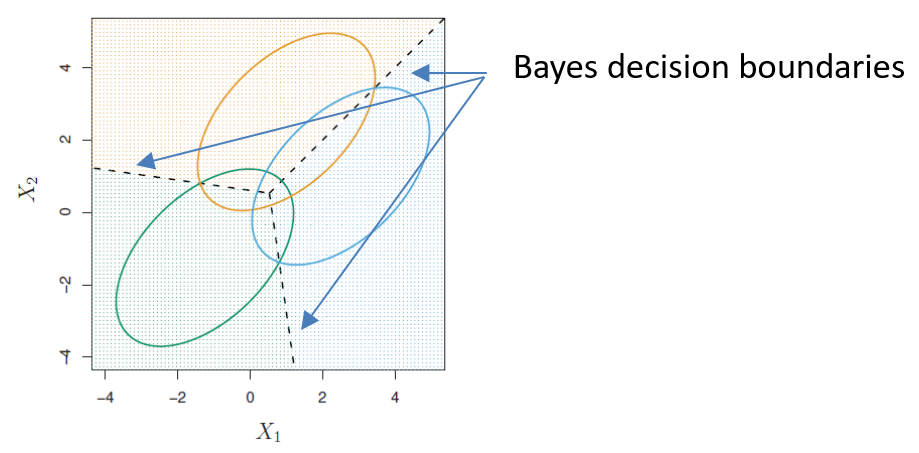
\includegraphics[width=.5\textwidth]{pictures/mlda}
	\end{center}
	LDA is optimized for minimum overall error, which is composed in a low sensitivity and a high specificity and you have to decide about a good threshold for yourself.

	\subsection{Quadratic discriminant analysis}
	In LDA it is assumed that the observations within each class are drawn from a multivariate Gaussian distribution with a class specific mean and a common covariance matrix. The Quadratic discriminant analysis (QDA) allows for each class to have its own covariance matrix. The main effect is, that the discriminant functions per class for a given observation x change to include a quadratic term.
	\begin{equation}
	\begin{split}
		X&\sim N(\mu_{k},\Sigma_{k})\\
		\delta_{k}(x)&=-\frac{1}{2}(x-\mu_{k})^T\Sigma_{k}^-1(x-\mu_{k})-\frac{1}{2}log|\Sigma_{k}|+log\pi_{k}\\
		&=-\frac{1}{2}x^T\Sigma_{k}^{-1}\mu_{k}-\frac{1}{2}\mu_{k}^T\Sigma_{k}^{-1}\mu_{k}-\frac{1}{2}log|\Sigma_{k}|+log\pi_{k}
	\end{split}
	\end{equation}
	Otherwise QDA uses the same steps as LDA, but instead of estimating a common covariance matrix, for each class a covariance matrix must be estimated. Once these parameters are known, for each class the corresponding discriminant function is evaluated and the test sample x is associated with the class that has the highest value.\\
	\begin{itemize}
		\item LDA has fewer parameters, hence it is less flexible, this tends to reduce the variance but increase the bias.
		\item QDA has more parameters, K covariance matrices instead of one, so you need K times more data. This increases the variance but decreases the bias
		\item With little training data use LDA, otherwise QDA
	\end{itemize}

	\subsection{A comparison of classification methods}

	\paragraph{Logistic regression vs. LDA}
	\begin{itemize}
		\item They often have very similar performance
		\item LDA tends to outperform logistic regression if the Gaussian assumption is approximately correct.
		\item Logistic regression tends to outperform LDA if the Gaussian assumption is basically wrong.
	\end{itemize}

	\paragraph{KNN}
	\begin{itemize}
		\item This is a non-parametric scheme, hence no model is assumed but simply a vote among the N nearest neighbors is performed to classify a test sample x.
		\item Hence one would expect KNN to outperform LDA and logistic regression if the decision boundaries need to be non-linear
		\item But KNN does not tell us which predictors are important and need lots of training data
	\end{itemize}

	\paragraph{QDA}
	\begin{itemize}
		\item In some sense this is a compromise between simple linear boundaries of LDA/logistic regression and arbitrary boundaries of KNN
		\item Here the boundaries are hyper-parabolas, which are much more complicated than hyperplanes but still much less flexible than KNN boundaries
		\item Hence it does take more training data than the linear methods but much less than KNN to perform well
	\end{itemize}

\end{document}
